\label{marco_teo}

En este capítulo se describirá el modelo en el cual se basa toda la investigación, también se definirán los conceptos utilizados a lo largo del trabajo como la definición de la presión social y los "blocking clusters". Además se comentará el algoritmo de integración temporal utilizado en la evolución temporal de cada proceso. 

\section{\label{sfm}Modelo de Fuerza social}

El modelo de "fuerza social" básico considera a los individuos como partículas auto-impulsadas. El movimiento de de los individuos está dominado por tres tipos de fuerzas de naturaleza diferente: la fuerza de deseo (autopropulsión), fuerzas sociales (repulsión) y fuerzas granulares (rozamiento). Se tienen en cuenta la interacción entre individuos y la interacción individuo-pared. Todas estas serán detalladas más adelante.   \\

Las fuerzas del modelo básico ingresan a una ecuación de movimiento (ley de Newton) de la forma de Ec. (\ref{newton}); de esta manera queda expresada la variación de velocidad en el tiempo que siente un individuo. El término $\mathbf{f}^{(ij)}$ es la interacción entre individuos; mientras que $\mathbf{f}^{(iW)}$ refleja la interacción con las paredes. Ambos términos contemplan tanto a la repulsión como al rozamiento. $\mathbf{f}_d^ {(i)}(t)$ es la fuerza de deseo. La ecuación de movimiento viene dado por $v_{i}(t)=d\mathbf{r_i}/dt$.

\begin{equation}
m_i\frac{d\mathbf{v_i}}{dt}=\mathbf{f}_d^ {(i)}(t)+ \sum_{i\neq j}^{N}\mathbf{f}^{(ij)} + \sum_{W}^{N}\mathbf{f}^{(iW)}
\label{newton}
\end{equation} 

La fuerza de deseo: es la fuerza que expresa el hecho de que cada persona es capaz de  acelerar o desacelerar hasta alcanzar la velocidad en que se siente más cómoda. La magnitud de esta velocidad se corresponde con el nivel de ansiedad que tenga por llegar a cierto lugar. La expresión matemática de esta fuerza viene dada por la fórmula~\ref{fdeseo}. Esta fórmula refleja el hecho que el individuo i-esimo, que posee masa $m_i$, desea  moverse con una velocidad $v_d^ {(i)}(t)$ en una dirección $\hat{\mathbf{e}}_d^ {(i)}(t)$, por lo tanto readapta su velocidad $\mathbf{v}_i(t)$ con un cierto tiempo característico $\tau$.

\begin{equation}
\mathbf{f}_d^ {(i)}(t)=m_i\,\displaystyle\frac{v_d^ {(i)}(t)\,\hat{\mathbf{e}}_d^ {(i)}(t)-\mathbf{v}_i(t)}{\tau}\label{fdeseo}
\end{equation}
\\

La repulsión social: es una fuerza que describe la tendencia que tienen las personas a mantenerse alejadas unas de otras. Depende de la distancia de separación entre individuos $d_{ij}=\left\|\mathbf{r_i}-\mathbf{r_j}\right\|$ y está en la dirección normal $\mathbf{n}_{ij}=(\mathbf{r_i}-\mathbf{r_j})/d_{ij}$ (versor que apunta desde el individuo j al individuo i). Los peatones están en contacto si el valor de $d_{ij}$ es más chico que la suma de los radios $r_{ij}=(r_i+r_j)$. $A_i$ y 	$B_i$ son constantes que se determinan experimentalmente.

\begin{equation}
\mathbf{f}_s^{(ij)}=A_i\,e^{(r_{ij}-d_{ij})/B_i}\mathbf{n}_{ij}\label{fsocial}
\end{equation} 
\\

La fuerza de rozamiento: aparece cuando los individuos están en contacto; esta fuerza es es proporcional a la velocidad relativa entre los mismos $\Delta \mathbf{v}_{ij}=(\mathbf{v}_i-\mathbf{v}_j)$. La dirección tangencial está representada por $\mathbf{t}_{ij}=(-n_{ij}^2,n_{ij}^1)$.  $\kappa$ es una constante y $g(x)$ es una función nula cuando los individuos no se tocan $(r_{ij}<d_{ij})$ y toma el valor de su argumento en caso contrario. 
\begin{equation}
\mathbf{f}_g^{(ij)}=\kappa\,g(r_{ij}-d_{ij})\,\Delta \mathbf{v}_{ij}\cdot\mathbf{t}_{ij}\label{frozamiento}
\end{equation}

La interacción de los individuos con las paredes tiene un tratamiento similar al que se tiene con la interacción entre individuos. La expresión (\ref{fparedes}) agrupa tanto a la repulsión como al rozamiento de la interacción peatón-pared. Las variables que componen esta expresión son: $d_{iW}$ que es la distancia del i-esimo peatón con la pared W, $n_{iW}$ es la dirección perpendicular entre éstos y $t_{iW}$ la dirección tangencial.

\begin{equation}
\mathbf{f}^{iW}=A_ie^{(r_{i}-d_{iW})/B_i}\mathbf{n}_{iW}-\kappa g(r_{i}-d_{iW})\Delta \mathbf{v}_{i}\cdot\mathbf{t}_{iW}
\label{fparedes}
\end{equation} 

A partir de la ecuación de movimiento (\ref{newton}) y de las condiciones iniciales en posición y velocidad de los individuos, se determina la dinámica de los peatones a lo largo del tiempo.\\

Una magnitud relevante y utilizada para caracterizar las multitudes evacuando en estado de pánico es la presión que siente cada individuo. En el área de la dinámica molecular existen diversas formas de definir la "presión local"~\cite{lion}. Según Helbing, para sistemas bidimiensionales como el que tratamos nosotros, esta se define como la suma de fuerzas normales actuando sobre un individuo, dividido su perímetro~\cite{Helbing1}. Por lo tanto, se tiene una fuerza por unidad de longitud; esta misma se representa en la ecuación (\ref{phelbing}).
En la Ref.~\cite{Helbing1} se reporta que a valores de presión superiores a 1600 Nm$^{-1}$ los individuos se lastiman y se vuelven obstáculos inamovibles. En este trabajo no se tienen en cuenta los eventuales desmayos producidos por las altas presiones. 

\begin{equation}
P_i =\frac{1}{2\pi r_{i}} \sum_{j\neq i}^{N}\mathbf{f}_s^{(ij)} \cdot\mathbf{n}_{ij}
\label{phelbing}
\end{equation} 

En el apéndice se desarrolla una derivación de la presión local que utiliza el teorema del virial y da soporte teórico a la presión utilizada por Helbing.
En la sección \ref{verlet} se detallará el cómputo de integración temporal de la Ec. (\ref{newton}), mientras que en la Sección \ref{ci} se comentarán qué condiciones iniciales se eligieron para cada situación de escape. 


\section{Blocking Clusters}

Al analizar la evolución de los individuos en estado de pánico se observó que el flujo no era constante y que presentaba "saltos" asociados a "taponamientos". Resultó entonces apropiado definir 
el concepto de blocking cluster~\cite{Dorso1} para estudiar a los individuos más próximos a la puerta que satisfacen la condición de estar en contacto con ella.
Se lo define como un conjunto mínimo de individuos en contacto que va desde un punto de la pared hacia otro. Estos puntos están próximos a los costados de la puerta. En forma más rigurosa, si un cluster granular (cluster humano) se define como 
\begin{equation}
P_i \in C_g \Longleftrightarrow \exists j \in c_g ~/~ d_{ij}<(r_i+r_j)
\end{equation} 
Siendo $P_i$  la i-esima persona y $r_i$ su radio. Entonces el blocking cluster corresponde al subconjunto mínimo de individuos (del cluster granular) tal que se encuentran más cerca de la puerta y cuyas primer y última partículas están en contacto con la pared a ambos lados de la puerta.   
Aquellos peatones que conforman el blocking cluster son los responsables de bloquear la salida de los individuos que se encuentran detrás de ellos. Típicamente se observa que los blocking cluster formados en las evacuaciones tiene estructura de "arco" como el que se muestra en la Fig. \ref{bc}. Basta que un solo peatón deje de estar en contacto con sus vecinos para que el blocking cluster deje de estar constituido. Además, estas estructuras mínimas actúan como una barrera para los individuos que tienen detrás, impidiendo la evacuación de peatones. \\

En este trabajo consideramos dos definiciones adicionales referentes a los \textit{blocking clusters}: por un lado, si los extremos de este no están en contacto con la pared de separación de las puertas (pero sí con las otras paredes del mismo lado del recinto) lo llamamos \textit{big blocking cluster}. En cambio, si una de las paredes de contacto es la pared de separación entre puertas, entonces los llamamos \textit{small blocking cluster} (ver ejemplos en la Fig.~\ref{bc}).

\begin{figure}[H]
    \centering
    \subfloat[\textit{Big blocking cluster}]{
    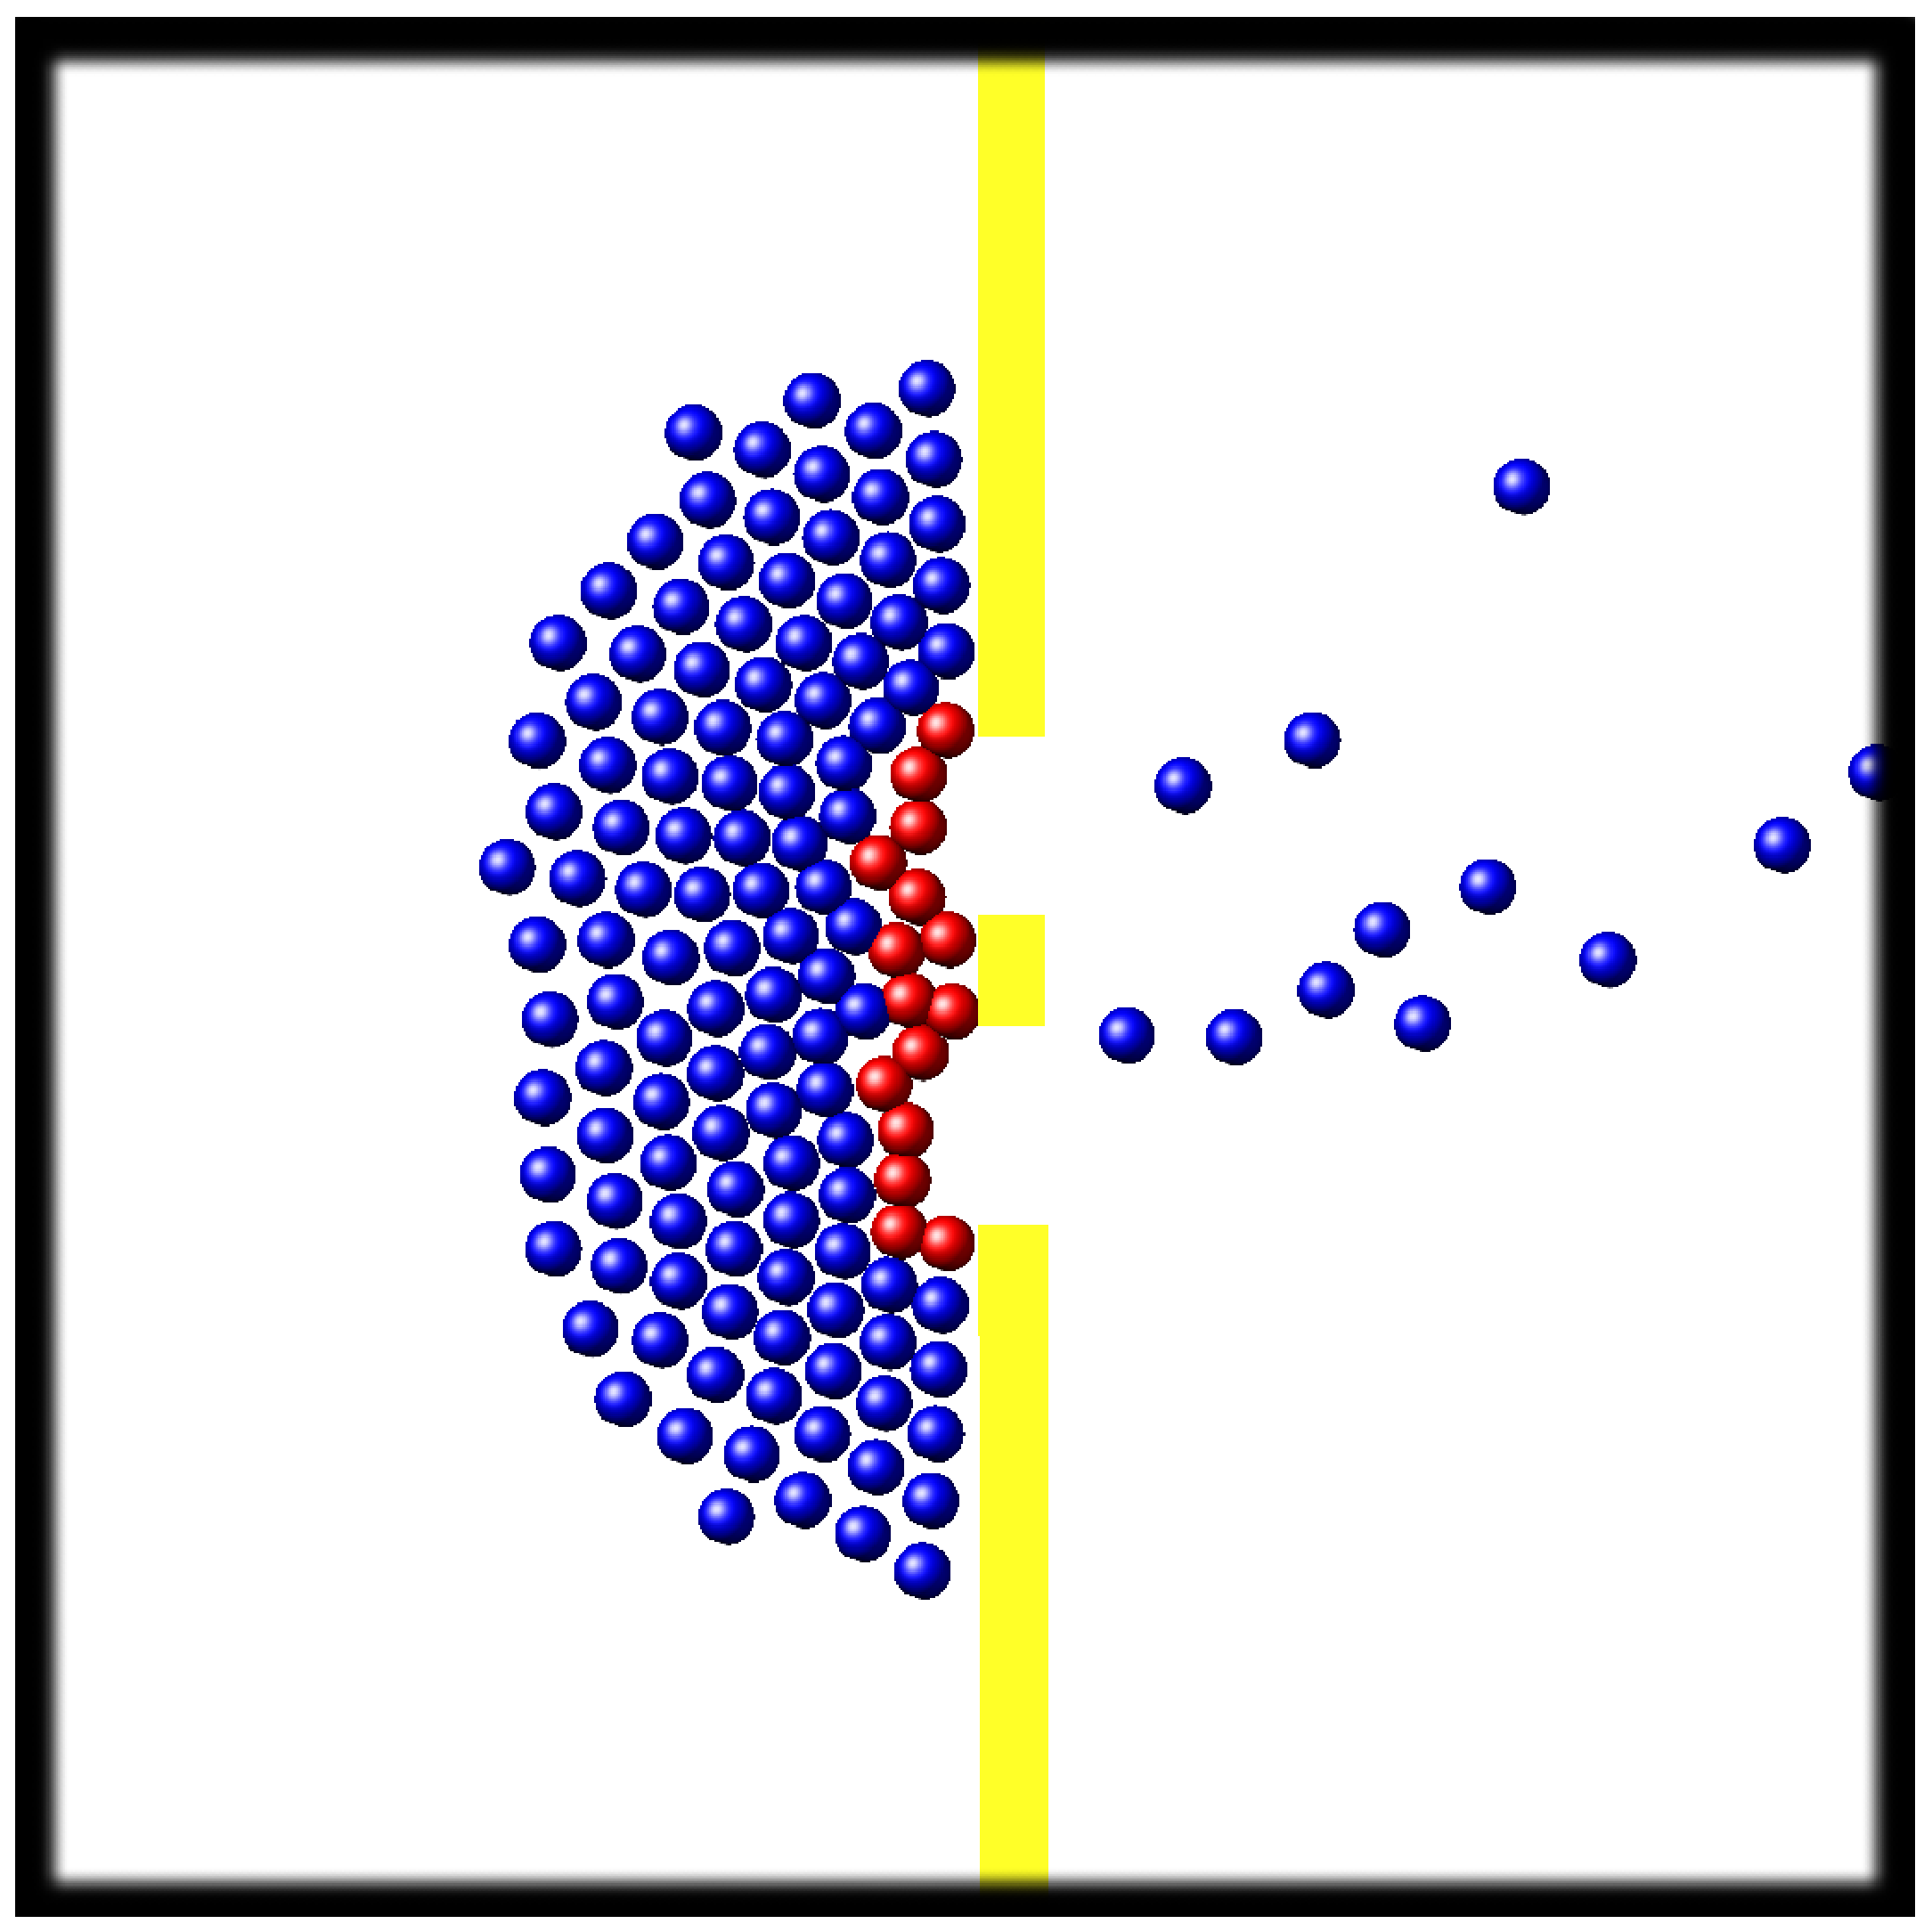
\includegraphics[width=7cm]{figuras/big_bc.eps}
    }\hfill
    \subfloat[\textit{Small blocking cluster}]{
    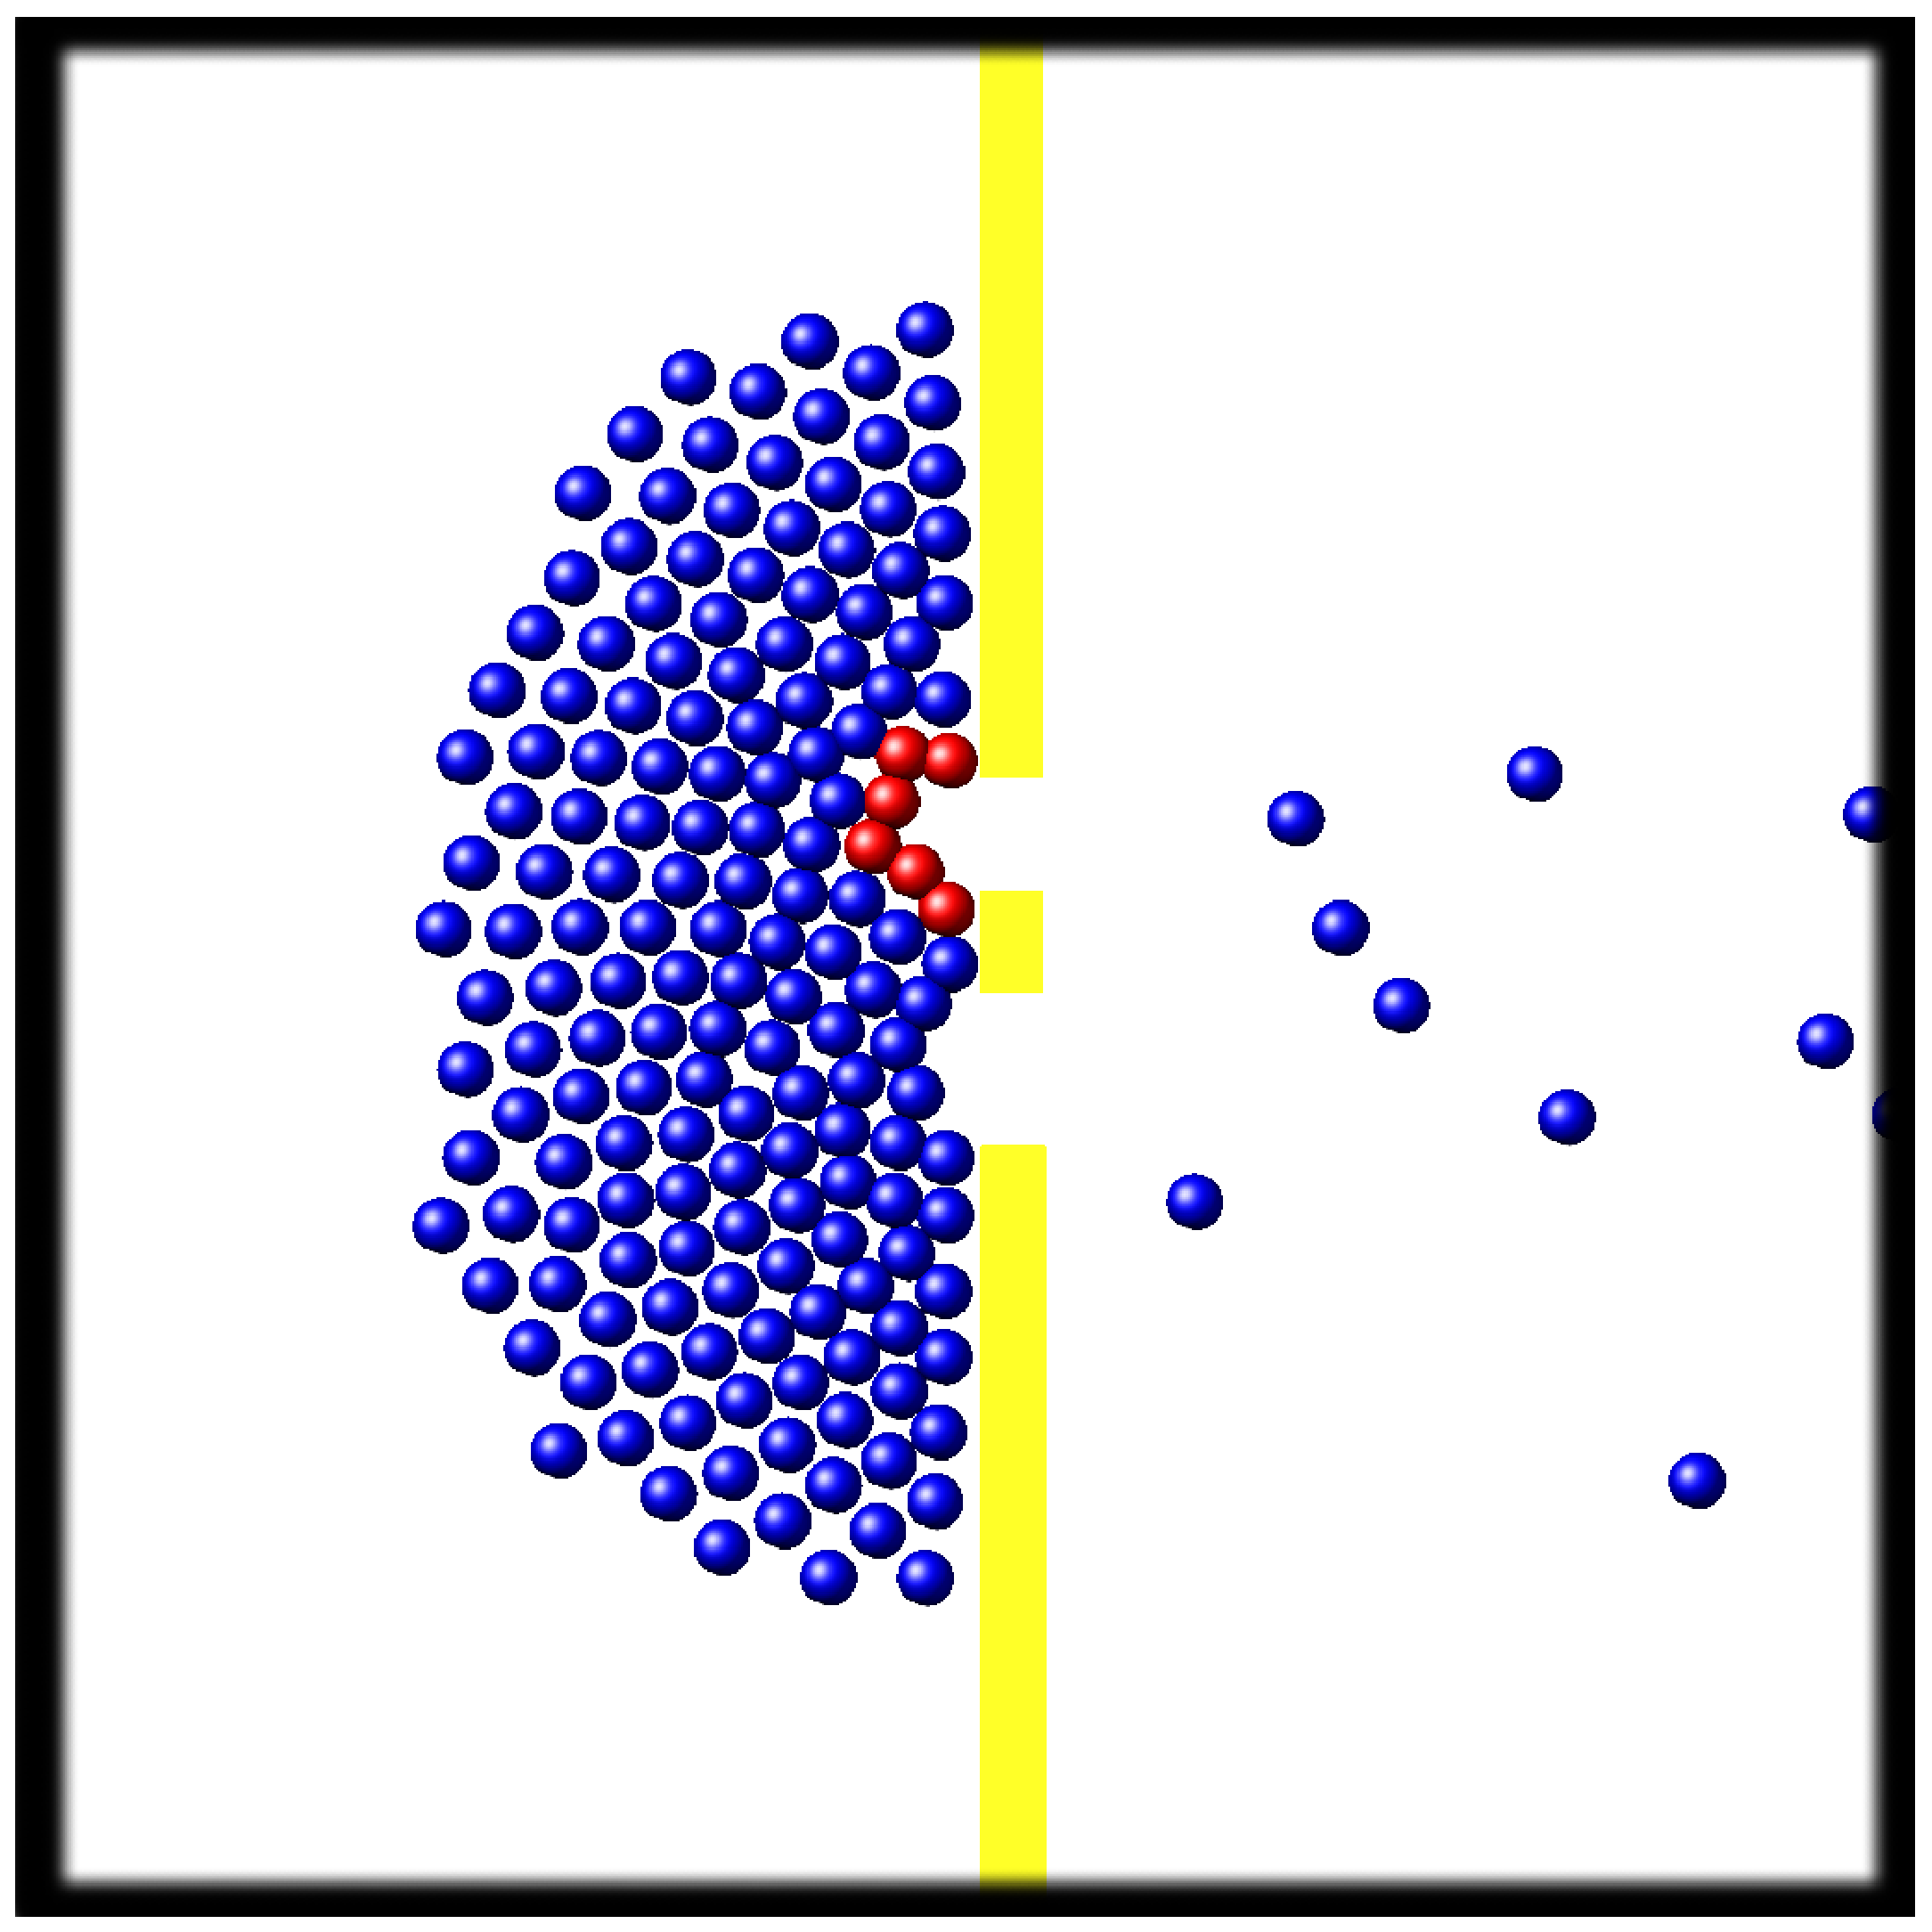
\includegraphics[width=7cm]{figuras/small_bc.eps}
    }
    \caption[width=5cm]{Imagen del proceso de evacuación de  200 individuos a través de dos puertas (velocidad de deseo $v_d=4\,$m/s). Las paredes se muestran en amarillo. Los inidividuos corresponden a las partículas en color azul. La salida de personas se produce de izquierda a derecha. Los \textit{blocking clusters} están identificados en color rojo. (a) se muestra un \textit{big blocking cluster}. La unión de individuos contempla las dos puertas. (b)  Se muestra un \textit{small blocking cluster} alrededor de la puerta superior.}
    \label{bc}
\end{figure}


\section{\label{verlet} Algoritmo de Verlet}

Para integrar las ecuaciones de movimiento se usó el algoritmo de Verlet en velocidades~\cite{haile}. Este método es ampliamente utilizado en el campo de dinámica molecular. Para esta forma de resolución, las ecuaciones que lo describen son:

\begin{equation}
x(t+\Delta t)=x(t)-v(t)\Delta t + \frac{1}{2}a(t)\Delta t^2 
\label{verlet_x}
\end{equation} 

\begin{equation}
v(t+\Delta t)=v(t)+\frac{a(t)+a(t+\Delta t)}{2}\Delta t
\label{verlet_v}
\end{equation}

El esquema de Verlet tiene un error de truncamiento local de ($\Delta t^2$). En la Fig. \ref{esquema_verlet} se muestra un diagrama del procedimiento, en donde se detalla la secuencia de actualización de variables para cada individuo. En el estado inicial disponemos únicamente de las posiciones y las velocidades de los individuos. Las aceleraciones se obtienen por medio de evaluación de las fuerzas $\mathbf{f}_d$, $\mathbf{f}_s$ y $\mathbf{f}_g$. Con estas magnitudes 
se calcula una nueva posición, se re-evalúan las fuerzas (aceleraciones) y se re-calcula la velocidad. Luego se vuelven a actualizar la posiciones y se repite el ciclo hasta construir las trayectorias de las partículas.
En la sección \ref{ci} del capítulo \ref{simulaciones} se detallarán las condiciones iniciales usadas en cada proceso de evacuación.\\

El algoritmo de Verlet es ampliamente utilizado por preservar las simetrías de las ecuaciones de Newton y las propiedades físicas de una gran cantidad de sistemas. Esto es gracias al hecho que tiene reversibilidad temporal y es simpléctico (conserva el volumen en el espacio de fases). En nuestro caso, esta propiedad es irrelevante porque la fuerza de deseo hace que no valga el teorema de Liouville. Además, es simple de implementar y posee buena estabilidad incluso para pasos temporales moderadamente grandes.

\begin{figure}[H]
    \centering
        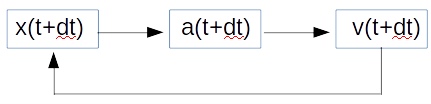
\includegraphics[scale=0.7]{figuras/esquema_verlet.png}
    \caption[width=5cm]{Esquema del procedimiento algorítmico de Verlet en velocidades}
    \label{esquema_verlet}
\end{figure}
